\chapter{Results}
\label{chp4}

\paragraph{ }In this chapter all results obtained from analysing the data and running the anomaly detection algorithms will be presented. 

\section{Beam Displacement Over Time}

\begin{figure}[!b]
	\begin{minipage}[b]{0.475\linewidth}
		\centering
		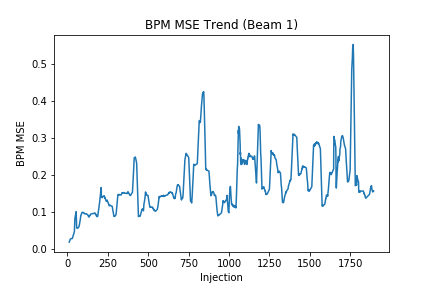
\includegraphics[width=\textwidth]{BPM_MSE_Trend_B1}
		\caption[BPM MSE Trend B1]{Trend Component of the BPM MSE for Beam 1}
		\label{fig::BPM_MSE_Trend_B1}
	\end{minipage}	
	\hspace{0.25cm}
	\begin{minipage}[b]{0.475\linewidth}
		\centering
		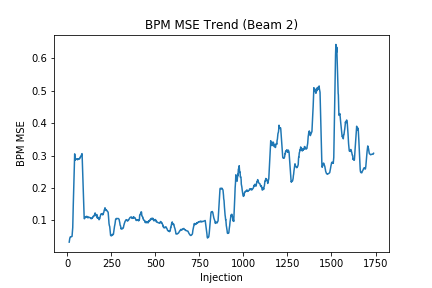
\includegraphics[width=\textwidth]{BPM_MSE_Trend_B2}
		\caption[BPM MSE Trend B2]{Trend Component of the BPM MSE for Beam 2}
		\label{fig::BPM_MSE_Trend_B2}
	\end{minipage}	
\end{figure}

\paragraph{ }When performing the initial analysis on the provided \acs{BPM} data, the \acs{MSE} of the Beam's Position with respect to its initial position in the first injection was calculated (refer to Section \ref{sec::Data_Cleaning_and_Analysis}). A rolling average of the time series points was taken to visualise the trend component. The window size was taken to be 12 since 12 injections are needed to fill the \acs{LHC}. Figures \ref{fig::BPM_MSE_Trend_B1} and \ref{fig::BPM_MSE_Trend_B2} show the trend component for Beam 1 and Beam 2 respectively. Although there's some noise in the data, it is clear from both plots that the Beam's position drifts with time.

\paragraph{ }This result confirms the suspicion that the beam's precision decreases over time. The cause of this phenomenon is due to ground motion as the slightest movement in one of the \acs{LHC}'s quadrupole magnets can throw off the beam's precision. Thus regular servicing and maintenance of the \acs{LHC} is important to reduce the number of anomalous injections.

\paragraph{ }First order differencing was then done on the data to remove the trend component. The resulting plots can be seen in Figures \ref{fig::BPM_MSE_Diff_B1} and \ref{fig::BPM_MSE_Diff_B2}. From these plots we can conclude that the spikes in the \acs{MSE} values are not seasonal but merely random.

\begin{figure}[!t]
	\begin{minipage}[b]{0.475\linewidth}
		\centering
		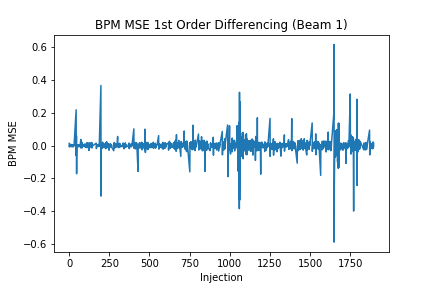
\includegraphics[width=\textwidth]{BPM_MSE_Diff_B1}
		\caption[BPM MSE Differencing B1]{1st Order Differencing for the BPM MSE for Beam 1}
		\label{fig::BPM_MSE_Diff_B1}
	\end{minipage}	
	\hspace{0.25cm}
	\begin{minipage}[b]{0.475\linewidth}
		\centering
		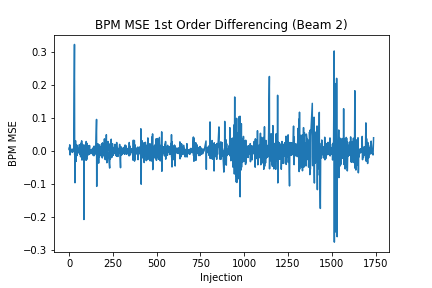
\includegraphics[width=\textwidth]{BPM_MSE_Diff_B2}
		\caption[BPM MSE Differencing B2]{1st Order Differencing for the BPM MSE for Beam 2}
		\label{fig::BPM_MSE_Diff_B2}
	\end{minipage}	
\end{figure}

